\section{Аналитический раздел}

В этом разделе будет приведено анализ в сфере организации футбольных турниров, выделено описание пользователей
Также проводится формализация поставленной задачи и формализация структуры данных.

\subsection{Анализ предметной области}

Футбольные турниры играют значительную роль в культурной и спортивной жизни общества, предоставляя участникам и зрителям возможность насладиться соревнованиями и создать собственные впечатления.

Футбольный турнир --- это соревнование, в котором несколько команд сражаются между собой, чтобы определить лучшую из них SRC.

Основная задача футбольного турнира заключается в создании среды для соревнования между командами с целью определения победителя и награждения его призом или званием чемпиона.

Турниры по футболу обычно проводятся в формате сезона, который на протяжении определенного периода времени, например, нескольких месяцев или года.
Команды получают очки за победы, ничьи или поражения, и в конце сезона команда с наибольшим количеством очков становится победителем.
Турнир по футболу привлекает внимание миллионов болельщиков по всему миру. В турнире участвуют команды из разных стран, состоящие из опытных профессионалов.

Основными правилами турнира по футболу являются:
\begin{itemize}
	\item каждая команда должна состоять из определенного числа игроков, обычно 11;
	\item цель игры: забивать голы в ворота соперника и не допускать голов в свои ворота;
	\item игра состоит из двух половинок по определенному времени, например, по 45 минут
	\item судья наблюдает за ходом игры и принимает решения в случае нарушений правил;
	\item побеждает команда, которая забила больше голов в течение игры.
\end{itemize}

\subsection{Формализация задачи}

Необходимо спроектировать базу данных для хранения информации о пользователях, турнирах, стадионах, матчах, отзывах и странах.
Требуется разработать программу с понятным интерфейсом для взаимодействия с информацией, хранящейся в базе данных.
В систему входят пять видов ролей --- гость, футболист, тренер, судья, администратор. 

\subsection{Формализация данных}

База данных должна хранить информацию о следующих сущностях:
\begin{itemize}
	\item пользователь;
	\item турнир;
	\item команда
	\item стадион;
	\item страна;
	\item матч;
	\item отзыв;
	\item заявка;
\end{itemize}

Сведения о каждой сущности проводится в таблице~\ref{tb:data}.

\begin{table}[ht]
	\begin{center}
		\begin{threeparttable}
			\caption{\label{tb:data} Сущности и их описания}
			\begin{tabular}{|c|p{10cm}|}
				\hline
				\textbf{Сущность} & \textbf{Описание} \\ \hline
				Пользователь & Логин, пароль, роль, фамилия, имя, возраст \\ \hline
				Турнир & Название, рейтинг, создатель, проводящая страна \\ \hline
				Стадион & Название, количество мест, страна \\ \hline
				Страна & Название, страна \\ \hline
				Команда & Название, создатель, страна \\ \hline
				Заявка & Время создания, создатель, команда, турнир \\ \hline
				Матч & Готевая команда, домашняя команда, голы гостевой, голы домашнней, турнир, стадион \\ \hline
				Отзыв & Пользователь, комментарий, оценка, турнир \\ \hline
			\end{tabular}
		\end{threeparttable}
	\end{center}
\end{table}

\newpage

На рисунке \ref{img:ERdiagram} приведена ER-диаграмма сущностей в нотации Чена.

\begin{figure}[h]
	\centering
	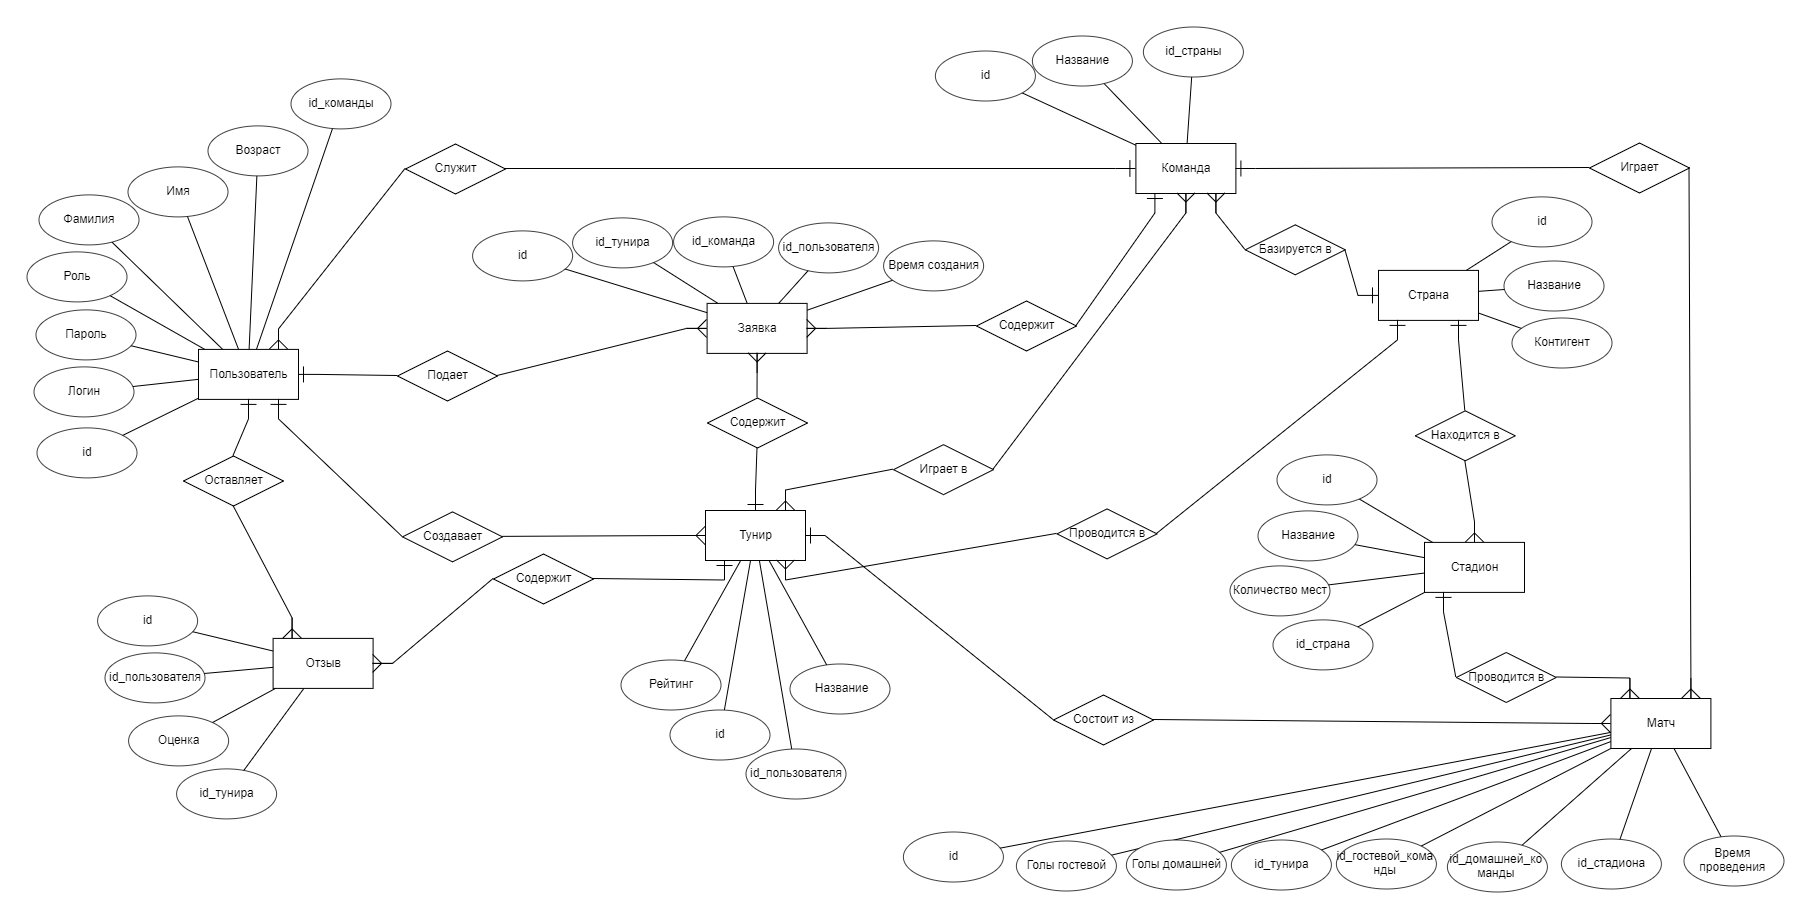
\includegraphics[height=0.3\textheight]{img/ER-diagram.png}
	\caption{ER-диаграмма сущностей}
	\label{img:ERdiagram}
\end{figure}
\subsection{Формализация пользовательских ролей}

Выделяются пять видов ролей:
\begin{itemize}
	\item гость --- неавторизованный пользователь, который обладающий возможностями зарегистрировать, входить в систему, просмотреть все данные турнира, оставить свои отзывы.
	\item футболист --- авторизованный пользователь, который может подать заявку на поступление в клуб, просмотреть все данные турнира.
	\item тренер --- авторизованный пользователь, который может принять/отменить заявку футболистов, подать заявку на поступление в турнир, просмотреть все данные турнира.
	\item судья --- авторизованный пользователь, который может создать свой турнир, принять/отменить заявку тренеров, вводить результаты матча.
	\item администатор --- пользователь, обладающий возможностями удалить/изменить данные пользователей, просмотреть все данные турнира.
\end{itemize}

На рисунках \ref{img:Use-case1}--\ref{img:Use-case2} приведена Use-Case диаграмма.

\begin{figure}[h]
	\centering
	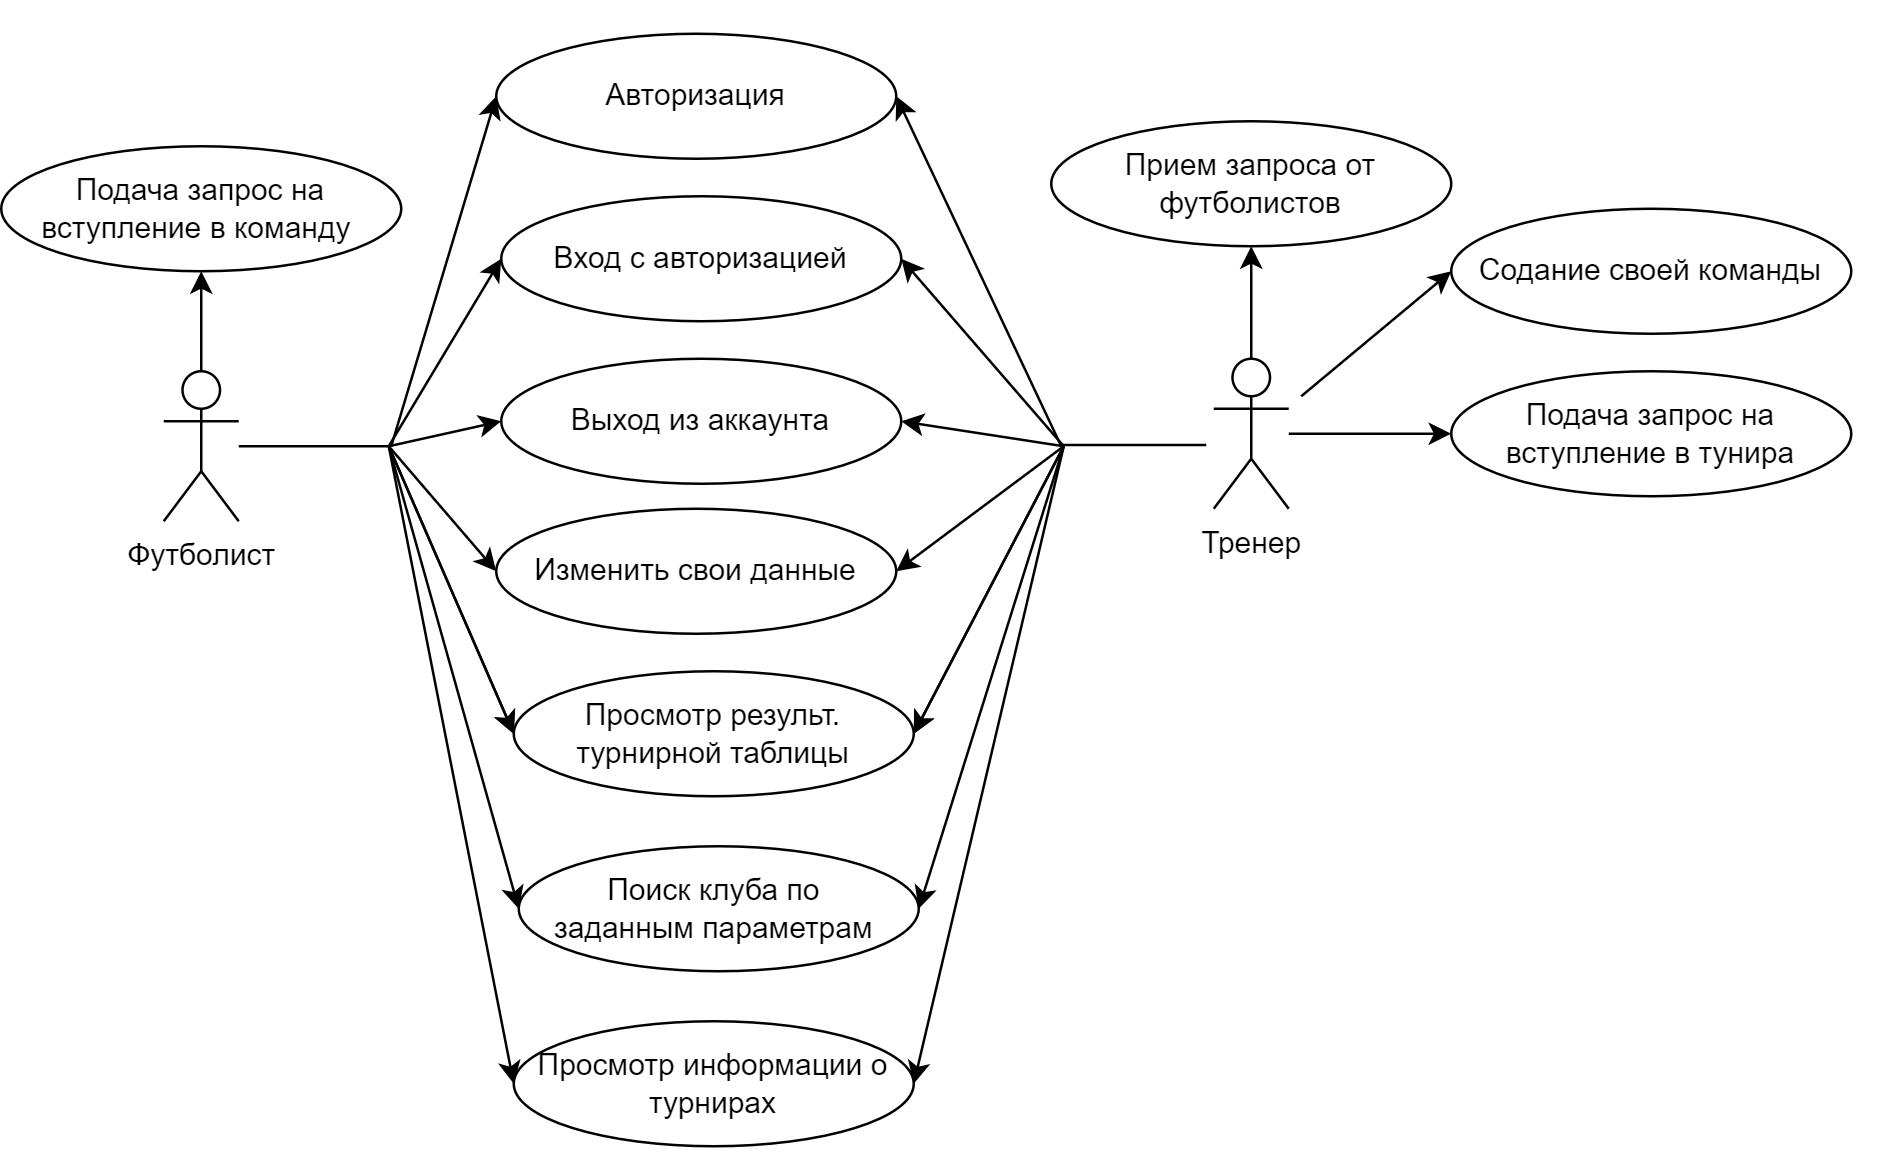
\includegraphics[height=0.3\textheight]{img/ppo-Use-Case1.png}
	\caption{Use-Case диаграмма}
	\label{img:Use-case1}
\end{figure}

\begin{figure}[h]
	\centering
	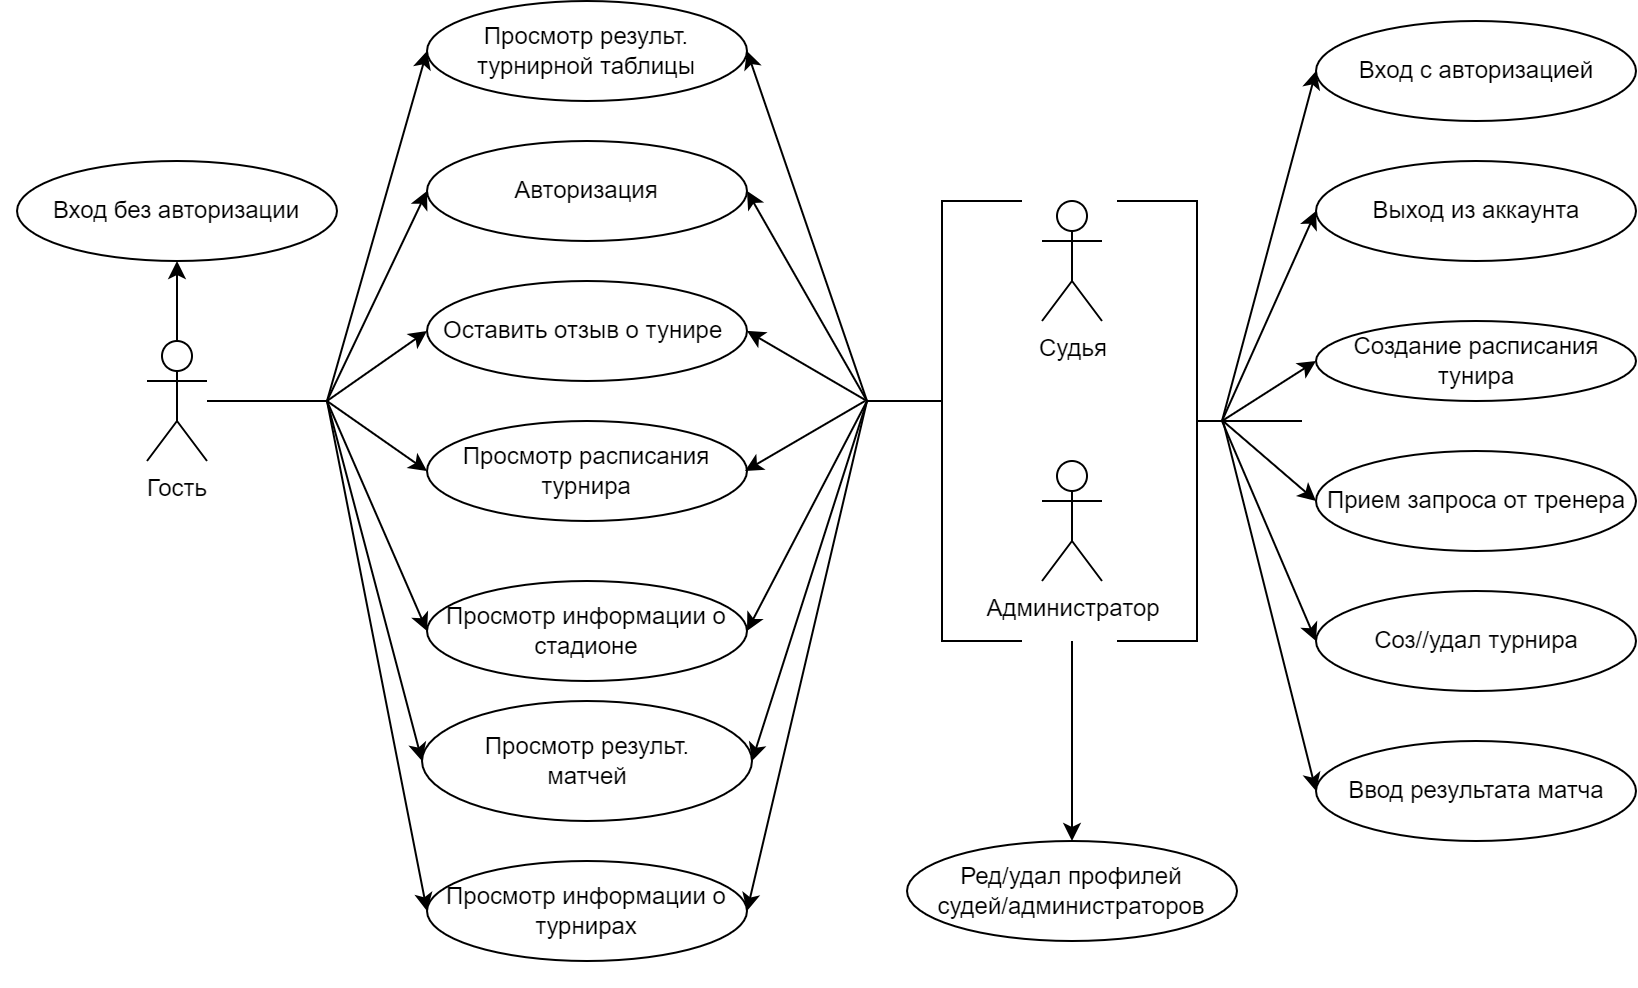
\includegraphics[height=0.3\textheight]{img/ppo-Use-Case2.png}
	\caption{Use-Case диаграмма (продолжение)}
	\label{img:Use-case2}
\end{figure}
\newpage

\subsection{Способ хранения полигональной модели}



\subsection*{Вывод}
В данном разделе была проанализирована предметная область, выделены ролевые модели системы, конкретизированы данные и их связь между собой, построены соответствующие диаграммы.